%%
%% This is file `mcmthesis-demo.tex',
%% generated with the docstrip utility.
%%
%% The original source files were:
%%
%% mcmthesis.dtx  (with options: `demo')
%%
%% -----------------------------------
%%
%% This is a generated file.
%%
%% Copyright (C)
%%       2010 -- 2015 by Zhaoli Wang
%%       2014 -- 2019 by Liam Huang
%%       2019 -- present by latexstudio.net
%%
%% This work may be distributed and/or modified under the
%% conditions of the LaTeX Project Public License, either version 1.3
%% of this license or (at your option) any later version.
%% The latest version of this license is in
%%   http://www.latex-project.org/lppl.txt
%% and version 1.3 or later is part of all distributions of LaTeX
%% version 2005/12/01 or later.
%%
%% This work has the LPPL maintenance status `maintained'.
%%
%% The Current Maintainer of this work is Liam Huang.
%%
%%
%% This is file `mcmthesis-demo.tex',
%% generated with the docstrip utility.
%%
%% The original source files were:
%%
%% mcmthesis.dtx  (with options: `demo')
%%
%% -----------------------------------
%%
%% This is a generated file.
%%
%% Copyright (C)
%%       2010 -- 2015 by Zhaoli Wang
%%       2014 -- 2019 by Liam Huang
%%       2019 -- present by latexstudio.net
%%
%% This work may be distributed and/or modified under the
%% conditions of the LaTeX Project Public License, either version 1.3
%% of this license or (at your option) any later version.
%% The latest version of this license is in
%%   http://www.latex-project.org/lppl.txt
%% and version 1.3 or later is part of all distributions of LaTeX
%% version 2005/12/01 or later.
%%
%% This work has the LPPL maintenance status `maintained'.
%%
%% The Current Maintainer of this work is Liam Huang.
%%
\documentclass{hci}
\usepackage{indentfirst}
%%\usepackage{CTeX}
\setlength{\parindent}{2em}
\pmsetup{CTeX = false,   % 使用 CTeX 套装时,设置为 true
        tcn = 1854116 Mingzhi Zhu, 
        sheet = true, titleinsheet = true, keywordsinsheet = true,
        titlepage = true, abstract = true}
\usepackage{newtxtext}%\usepackage{palatino}
\usepackage{lipsum}
%\usepackage[notref,notcite]{showkeys}
\title{Lab1: Automatic Speech Recognition}
\author{1854116 \\Mingzhi Zhu}
\date{Xiaosi Voice Assistant\\\today}
\begin{document}

\maketitle
\tableofcontents
\newpage
%% Generate the Table of Contents, if it's needed.
%% \tableofcontents
%% \newpage
%%
%% Generate the Memorandum, if it's needed.
%% \memoto{\LaTeX{}studio}
%% \memofrom{Liam Huang}
%% \memosubject{Happy \TeX{}ing!}
%% \memodate{\today}
%% \logo{\LARGE I'm pretending to be a LOGO!}
%% \begin{memo}[Memorandum]
%%   \lipsum[1-3]
%% \end{memo}
%%
\section{Modifications}

\begin{itemize}
	\item After two weeks of structural analysis of \underline{asr.py/asrinterface.py}, the user interface was partially changed in this lab, and Qt Designer was used to layout the interface.
	\item Now the new program provides two ways to wake up the voice assistant,one is clicking the Siri iron and the other is saying something when Siri iron is moving.
	\item This program uses Baidu speech recognition API instead of PocketSphinx.
\end{itemize}
\subsection{GUI}
\subsubsection{Window Icon and Name}
I changed the name and icon of the windows to make them more beautiful and conform to the overall style of Xiaosi voice assistant.The picture is shown in \textbf{figure1}.
 
% TODO: \usepackage{graphicx} required
\begin{figure}[htb]
	\centering
	
\includegraphics[width=0.7\linewidth]{../picture/1}
	\caption{Window Icon and Name}
	\label{figure1}
\end{figure}

\subsubsection{Main Interface}
Main interface is also startup interface.The top-down composition of the user interface is described below.
\begin{itemize}
	\item \textbf{Windows Name:}Define the window name of app.
	\item \textbf{Title:}Explain to the user that this is a helper program.
	\item \textbf{Clickable Button:}A gif file called \textit{siri-ianzhao.gif} in folder \textit{assets}.
	\item \textbf{Text Echo:}Show state of the assistant. Such as listening,pardon or what user said.
	\item \textbf{Tips:}Prompt the user to use the voice assistant by saying the following command.
\end{itemize}
The specific interface is shown in \textbf{\ref{figure4}}.


\subsubsection{Wake-up Logic}
You have two ways to activate the assistant.
\begin{itemize}
	\item \textbf{Click Button:}Click the Siri icon on the interface to wake up voice assistant.The iron is shown in \textbf{figure2}.
	\begin{figure}[htb]
		\centering
		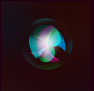
\includegraphics[width=0.1\linewidth]{../picture/3}
		\caption{Button Icon}
		\label{figure2}
	\end{figure}
	\item \textbf{Say Directly}Say someting to wake up voice assistant,for example you can say "soushuozhongwen" and the result is shown in \textbf{figure3}.
		
\end{itemize}


% TODO: \usepackage{graphicx} required
\begin{figure}[htb]
	\centering
	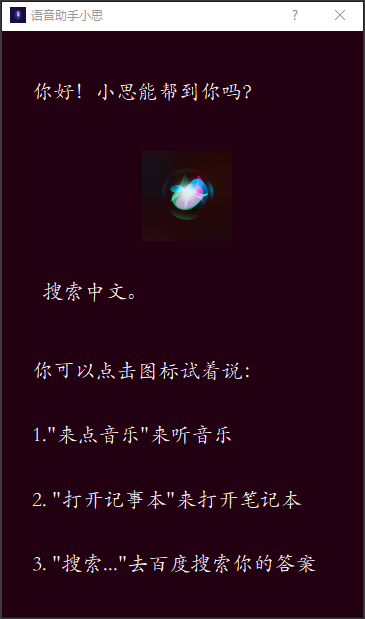
\includegraphics[width=0.5\linewidth]{../picture/4}
	\caption{Say Something}
	\label{figure3}
\end{figure}

\subsection{Code}
\subsubsection{Interface code}
\begin{itemize}
	\item \textbf{QLabel}
	\begin{figure}[htb]
		\centering
		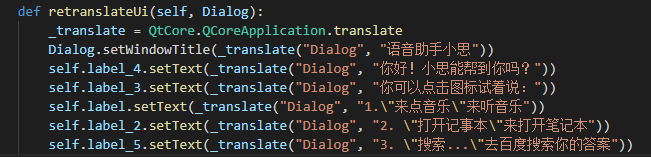
\includegraphics[width=0.9\linewidth]{../picture/5}
		\label{figure5}
	\end{figure}
	\item \textbf{QIron}
	\begin{figure}[h!]
		\centering
		
\includegraphics[width=0.9\linewidth]{../picture/7}
		\label{figure7}
	\end{figure}
    \newpage
	\item \textbf{QMovie}
	\begin{figure}[h!]
		\centering
		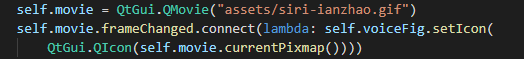
\includegraphics[width=0.9\linewidth]{../picture/6}
		\label{figure6}
	\end{figure}
	
\end{itemize}

\begin{figure}[htb]
	\centering
	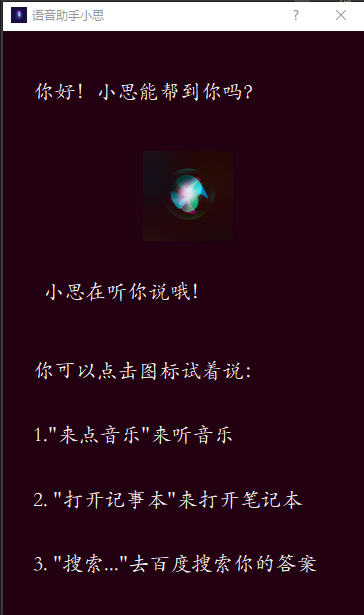
\includegraphics[width=0.5\linewidth]{../picture/2}
	\caption{Main Interface}
	\label{figure4}
\end{figure}
\subsubsection{Speech Recognition}
\begin{itemize}
	\item \textbf{Voice Recording:}Use function in SpeechRecognition package to monitor to user's microphone. It will stop automatically when no further detection.The core code is shown below, and the detailed implementation is shown in the code file \underline{recorder.py}.
    \begin{figure}[h!]
    	\centering
    	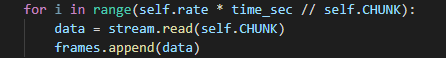
\includegraphics[width=0.9\linewidth]{../picture/8}
    	\label{figure8}
    \end{figure}
	\newpage
	\begin{figure}[htb]
		\centering
		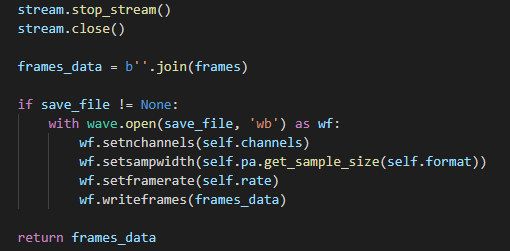
\includegraphics[width=0.9\linewidth]{../picture/9}
		\label{figure9}
	\end{figure}
	\item \textbf{Voice Recognition:}Use BaiduAip to recognize the voice.Register an account on Baidu AI console, apply for a key for speech recognition, and call the interface provided by Baidu locally.The core code is shown below, and the detailed implementation is shown in the code file \underline{asr.py}.
	\begin{figure}[htb]
		\centering
		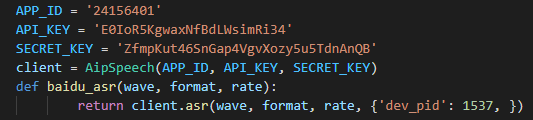
\includegraphics[width=0.9\linewidth]{../picture/10}
		\label{figure10}
	\end{figure}
\end{itemize}

\subsubsection{Command Execution}
\begin{itemize}
	\item \textbf{Keyword Retrieval:}Retrieve the keywords in the text returned by Baidu API. If the keywords are consistent with the keywords in the command, execute the command.The core code is shown below, and the detailed implementation is shown in the code file \underline{app.py}.
	\begin{figure}[h!]
		\centering
		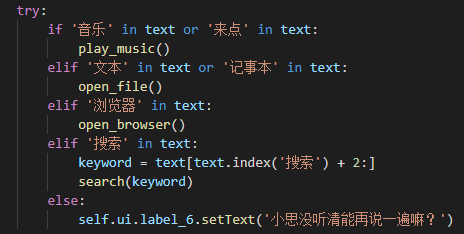
\includegraphics[width=0.8\linewidth]{../picture/12}
		\label{figure11}
	\end{figure}
	\item \textbf{Not Continuous Execution:}After recognizing the voice and retrieving the voice for 2S, the next voice command execution starts. The purpose of this operation is to give users enough time to get the text feedback on the interface.The core code is shown below, and the detailed implementation is shown in the code file \underline{app.py}.
	\begin{figure}[htb]
		\centering
		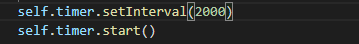
\includegraphics[width=0.8\linewidth]{../picture/13}
		\label{figure12}
	\end{figure}
\end{itemize}

\subsubsection{Assistant Functions}
I add four functions to the program,they are: 
\begin{itemize}
	\item Play Music
	\item Open File
	\item Search on Baidu
	\item Open Browser
\end{itemize}
The core code is shown below, and the detailed implementation is shown in the code file \underline{app.py}.
\begin{figure}[htb]
	\centering
	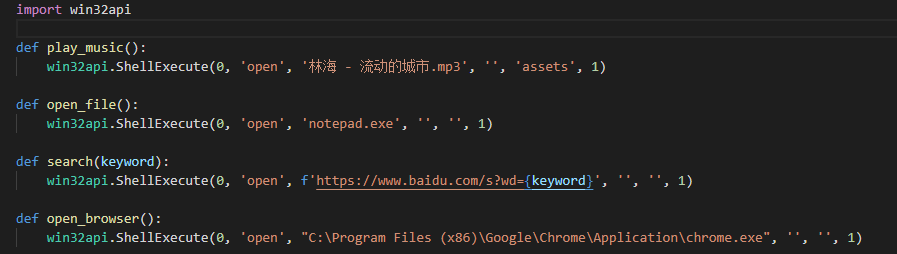
\includegraphics[width=0.9\linewidth]{../picture/11}
	\label{figure13}
\end{figure}

\section{Discussion}
\subsection{Accuracy of Speech Recognition}
The speech recognition effect of Sphinx interface is very poor. Although it supports Chinese recognition, it can hardly recognize the user's command accurately, so I use Baidu speech recognition API instead.The advantage of Baidu API is that it has complete documentation to teach you how to call their interfaces in Python programs. And the recognition accuracy is 95\% according to the official documents. In the actual experience, the API recognition result is very accurate.Baidu API recognition speed is also very fast,I  can hardly feel that this is an online interface.

But Baidu API also has its shortcomings,Baidu API only has limited call opportunities, and Sphinx is a completely free api.Baidu API is an online interface, once the computer does not access to the Internet, speech recognition programs can not run.In particular, Baidu API can not be used when the computer uses proxy IP address.

The console interface of Baidu API is shown in \textbf{figure5}.
\begin{figure}[htb]
	\centering
	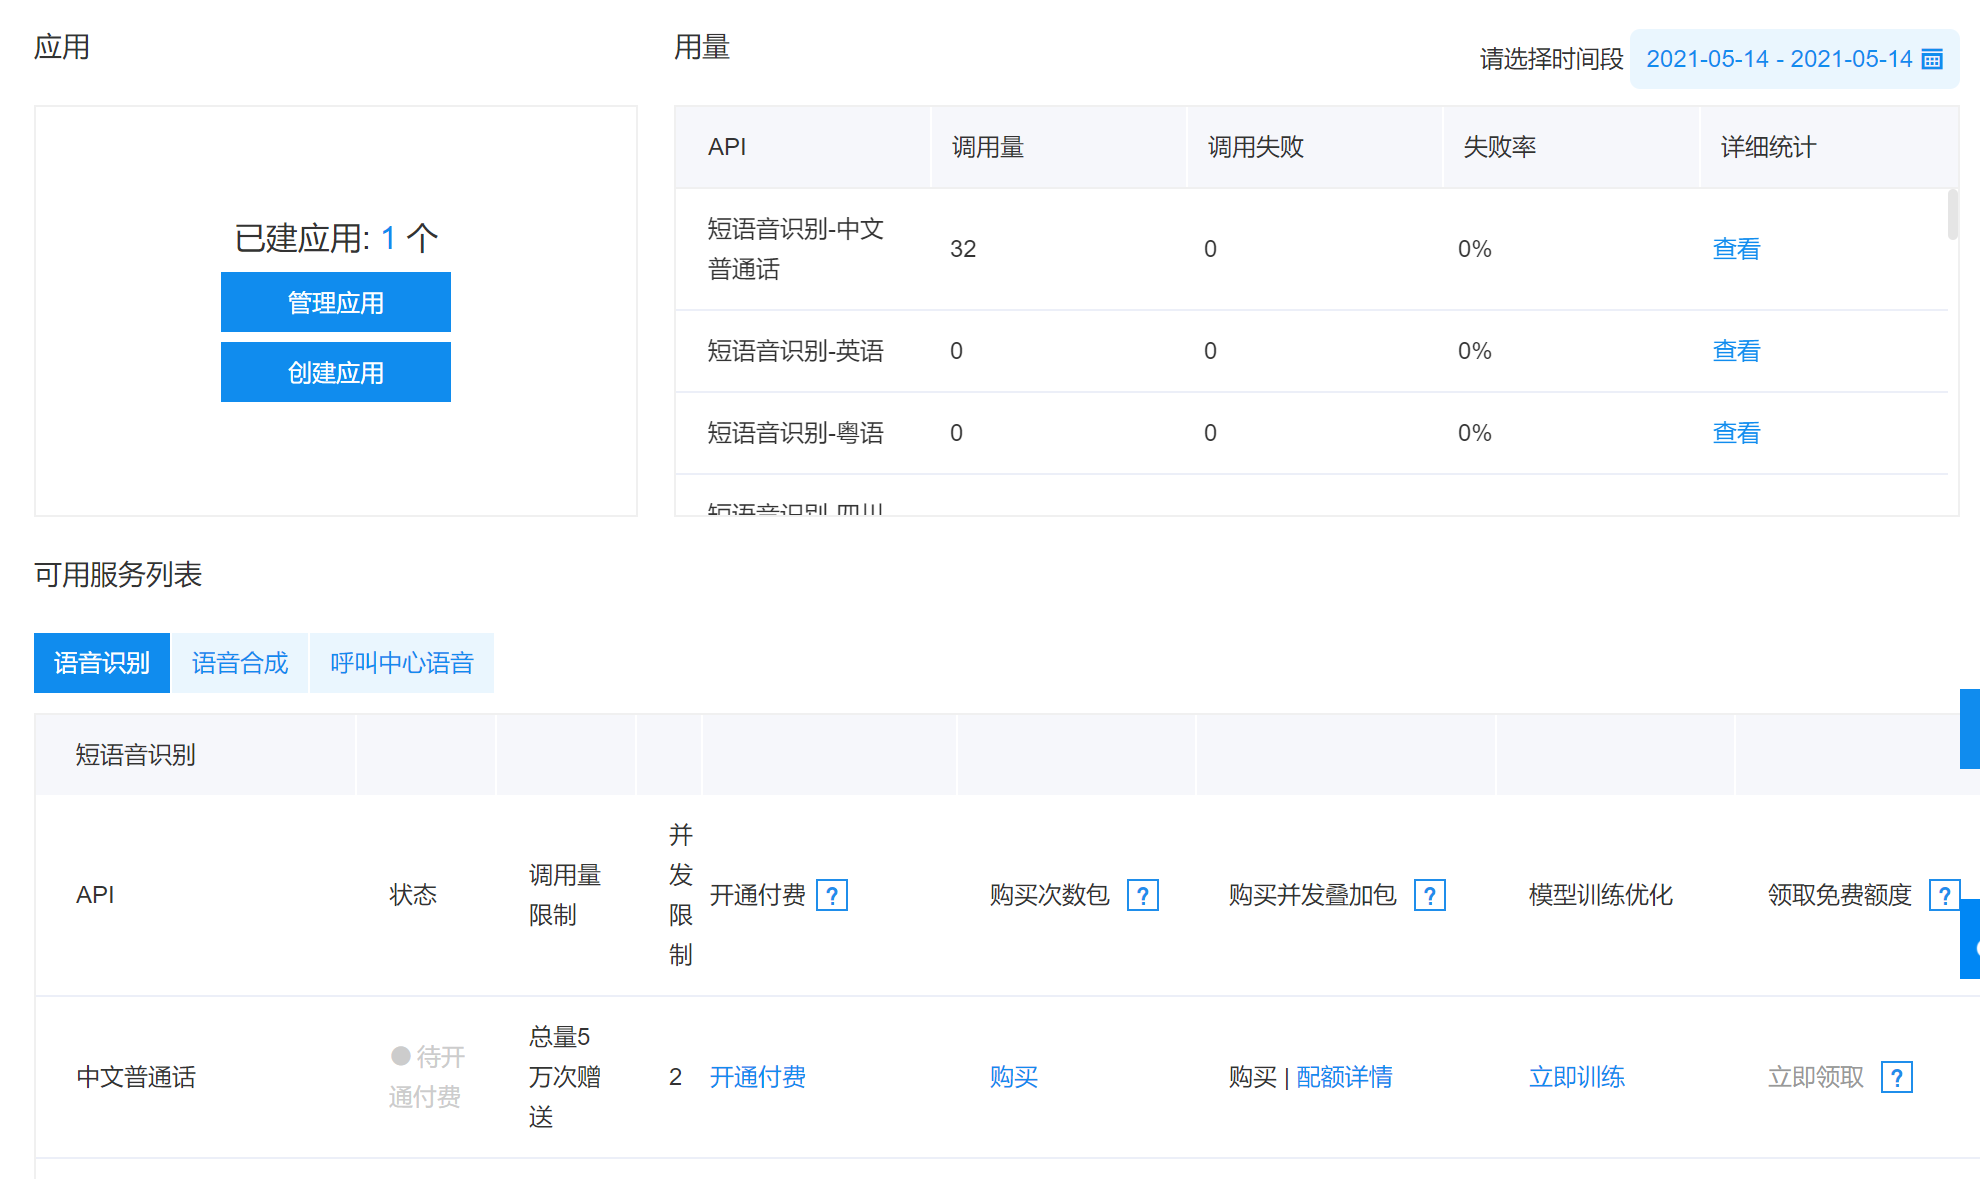
\includegraphics[width=1\linewidth]{../picture/14}
	\caption{Console of Baidu API}
	\label{figure15}
\end{figure}
\subsection{Audio Recording Quality}
Pyaudio package supports multi sampling rate and multi-channel audio format, while SpeechRecognition package only supports mono audio.At the same time, SpeechRecognition package supports silent automatic stop, while PyAudio needs to set recording time manually.

So I use the \textbf{adjust\_for\_ambient\_noise} function in PyAudio called every 0.5 seconds to ensure the audio recording quality.In addition, I set the sampling rate to 16000 while mono recording.

\begin{thebibliography}{99}
\bibitem{1} Designing the User Interface: Strategies for Effective Human-Computer Interaction, 6th edition,Ben Shneiderman,Catherine Plaisant,Maxine Cohen
\bibitem{2} Baidu Speech Recognition Technology Document,\url{https://cloud.baidu.com/doc/SPEECH/index.html}
\end{thebibliography}

\end{document}
%%
%% This work consists of these files mcmthesis.dtx,
%%                                   figures/ and
%%                                   code/,
%% and the derived files             mcmthesis.cls,
%%                  command execution                 mcmthesis-demo.tex,
%%                                   README,
%%                                   LICENSE,
%%                                   mcmthesis.pdf and
%%                                   mcmthesis-demo.pdf.
%%
%% End of file `mcmthesis-demo.tex'.
